\documentclass{ctexart}

\usepackage{appendix}
\usepackage{listings}% 插入代码
\usepackage{xcolor} 
\usepackage{graphicx}% 插入表格/图片
\usepackage{booktabs} % 绘制表格
\usepackage{caption} % 标题
\usepackage{geometry}
\usepackage{array}
\usepackage{amsmath}
\usepackage{subfigure} % 插入图片
\usepackage{longtable}
\usepackage{abstract}% 摘要
\pagestyle{plain} % 页眉消失
\usepackage{setspace}
\usepackage{multirow}% 表格
\usepackage{diagbox}
\usepackage{enumerate}% 序号
\usepackage{float}% 固定图片或表格的位置
\usepackage{gensymb}
\usepackage{microtype}

\geometry{a4paper,left=2.5cm,right=2.5cm,top=2cm,bottom=2cm}% 页边距
\lstset{
    numbers=left, % 设置行号位置
    numberstyle=\tiny, % 设置行号大小
    keywordstyle=\color{blue}, % 设置关键字颜色
    commentstyle=\color[cmyk]{1,0,1,0}, % 设置注释颜色
    escapeinside=``, % 逃逸字符(1左面的键),用于显示中文
    breaklines, % 自动折行
    extendedchars=false, % 解决代码跨页时,章节标题,页眉等汉字不显示的问题
    xleftmargin=1em,xrightmargin=1em, aboveskip=1em, % 设置边距
    tabsize=4, % 设置tab空格数
    showspaces=false % 不显示空格
}

\title{太阳能小屋的设计}
\date{}
\author{}

\begin{document}
    \maketitle
    \renewcommand{\abstractname}{\Large 摘要\\}
    \begin{abstract}
        \normalsize
        本文针对太阳能小屋设计问题,建立了多种优化模型。
        
        针对问题一,为达到最高收益,进行数据预处理,对光能进行积分以解决辐射量的计算问题,接下来分别计算每种电池板在每个墙面的收益,以最优的太阳能电池板铺设方式,包含墙面选择与铺设方式选择。然后进行串并联连接方式与变压器选择,最终得到了最高的发电量,与最大经济效益。
        
        针对问题二,
        
        针对问题三,
        
        \textbf{关键字}:优化
    \end{abstract}
    \newpage
% 重新设置页面边距
    \newgeometry{a4paper,left=3.18cm,right=3.18cm,top=2.54cm,bottom=2.54cm}
	\section{问题背景与重述}
	\subsection{问题背景}
    在设计太阳能小屋时,需在建筑物外表面(屋顶及外墙)铺设光伏电池,光伏电池组件所产生的直流电需要经过逆变器转换成220V交流电才能供家庭使用,并将剩余电量输入电网。不同种类的光伏电池每峰瓦的价格差别很大,且每峰瓦的实际发电效率或发电量还受诸多因素的影响,如太阳辐射强度、光线入射角、环境、建筑物所处的地理纬度、地区的气候与气象条件、安装部位及方式(贴附或架空)等。因此,在太阳能小屋的设计中,研究光伏电池在小屋外表面的优化铺设是很重要的问题。
    
    在求解每个问题时,都要求配有图示,给出小屋各外表面电池组件铺设分组阵列图形及组件连接方式(串、并联)示意图,也要给出电池组件分组阵列容量及选配逆变器规格列表。在同一表面采用两种或两种以上类型的光伏电池组件时,同一型号的电池板可串联,而不同型号的电池板不可串联。在不同表面上,即使是相同型号的电池也不能进行串、并联连接。应注意分组连接方式及逆变器的选配。
    
    根据附件 1 提供的信息,附件 2 和附件 3 提供的,以及附件 4 提供的,可以建立数学模型解决以下问题:
    
    \subsection{问题表述}
    \begin{enumerate}[(1)]
        \item 问题一:请根据山西省大同市的气象数据,仅考虑贴附安装方式,选定光伏电池组件,对小屋(见附件2)的部分外表面进行铺设,并根据电池组件分组数量和容量,选配相应的逆变器的容量和数量。
        \item 问题二:电池板的朝向与倾角均会影响到光伏电池的工作效率,请选择架空方式安装光伏电池,重新考虑问题1。
        \item 问题三:根据附件7给出的小屋建筑要求,请为大同市重新设计一个小屋,要求画出小屋的外形图,并对所设计小屋的外表面优化铺设光伏电池,给出铺设及分组连接方式,选配逆变器,计算相应结果。
    \end{enumerate}

    \section{问题分析}
    \subsection{问题一分析}
    对于问题一进行数据预处理,为了达成年太阳能光伏发电总量尽可能大,而单位发电量的费用尽可能小这两个目标,我们一步步地对

	因为附件4所给大同典型气象年气象数据为离散型数据
    \subsection{问题二分析}
    首先通过,设计相应的架空方式,确保最大的全年太阳能光伏发电总量,以获取更多的收益。
    \subsection{问题三分析}
    对于该问题,首先需要建立,需要设计接收阳光最优化的房子。基于太阳辐射,选择最优的房屋朝向角度及建筑设计。

    \section{模型假设}
    \begin{enumerate}[(1)]
        \item 在时间分布上,辐射度是连续的。
        \item 每年太阳辐射量基本不变。
        \item 基于
        \item 假设电池板不能重叠,且不能超出可用铺设区域。
    \end{enumerate}

    \section{符号说明}
    \begin{center}
        \setlength{\tabcolsep}{9mm}{
            \begin{tabular}{ccc}
                \toprule  % 添加表格头部粗线。
                \textbf{符号} & \textbf{意义} & \textbf{单位}\\
                \midrule  % 添加表格中横线
                \textbf{K} & \textbf{聚类类别数} & \textbf{}\\
                \textbf{W} & \textbf{意义} & \textbf{单位}\\
                \textbf{i} & \textbf{意义} & \textbf{}\\
                \textbf{j} & \textbf{意义} & \textbf{}\\
                \textbf{符号} & \textbf{意义} & \textbf{单位}\\
                \textbf{符号} & \textbf{意义} & \textbf{单位}\\
                \textbf{符号} & \textbf{意义} & \textbf{单位}\\
                \textbf{符号} & \textbf{意义} & \textbf{单位}\\
                \textbf{符号} & \textbf{意义} & \textbf{单位}\\
                \textbf{符号} & \textbf{意义} & \textbf{单位}\\
                \textbf{符号} & \textbf{意义} & \textbf{单位}\\
                \bottomrule % 添加表格底部粗线
        \end{tabular}}
    \end{center}

    \section{模型建立与求解}
    \subsection{问题一模型的建立与求解}
    因为
    \subsubsection{问题一模型的建立}
    针对

    
    为解决辐射量的计算问题,对光能进行积分
    
    为解决最优太阳能电池板问题,

    为解决太阳能电池板排布问题,建立了

    为解决变压器问题,优化出最低价格的变压器使用策略。
    

    
    \subsubsection{数据预处理}
    为了避免夜晚数据为0影响多项式拟合,首先剔除辐射强度为0的数据。

	接下来进行多项式拟合,拟合效果如下图所示。



	\begin{figure}[H] % [H] 表示强制当前位置插入图片
        \centering % 使图片居中
        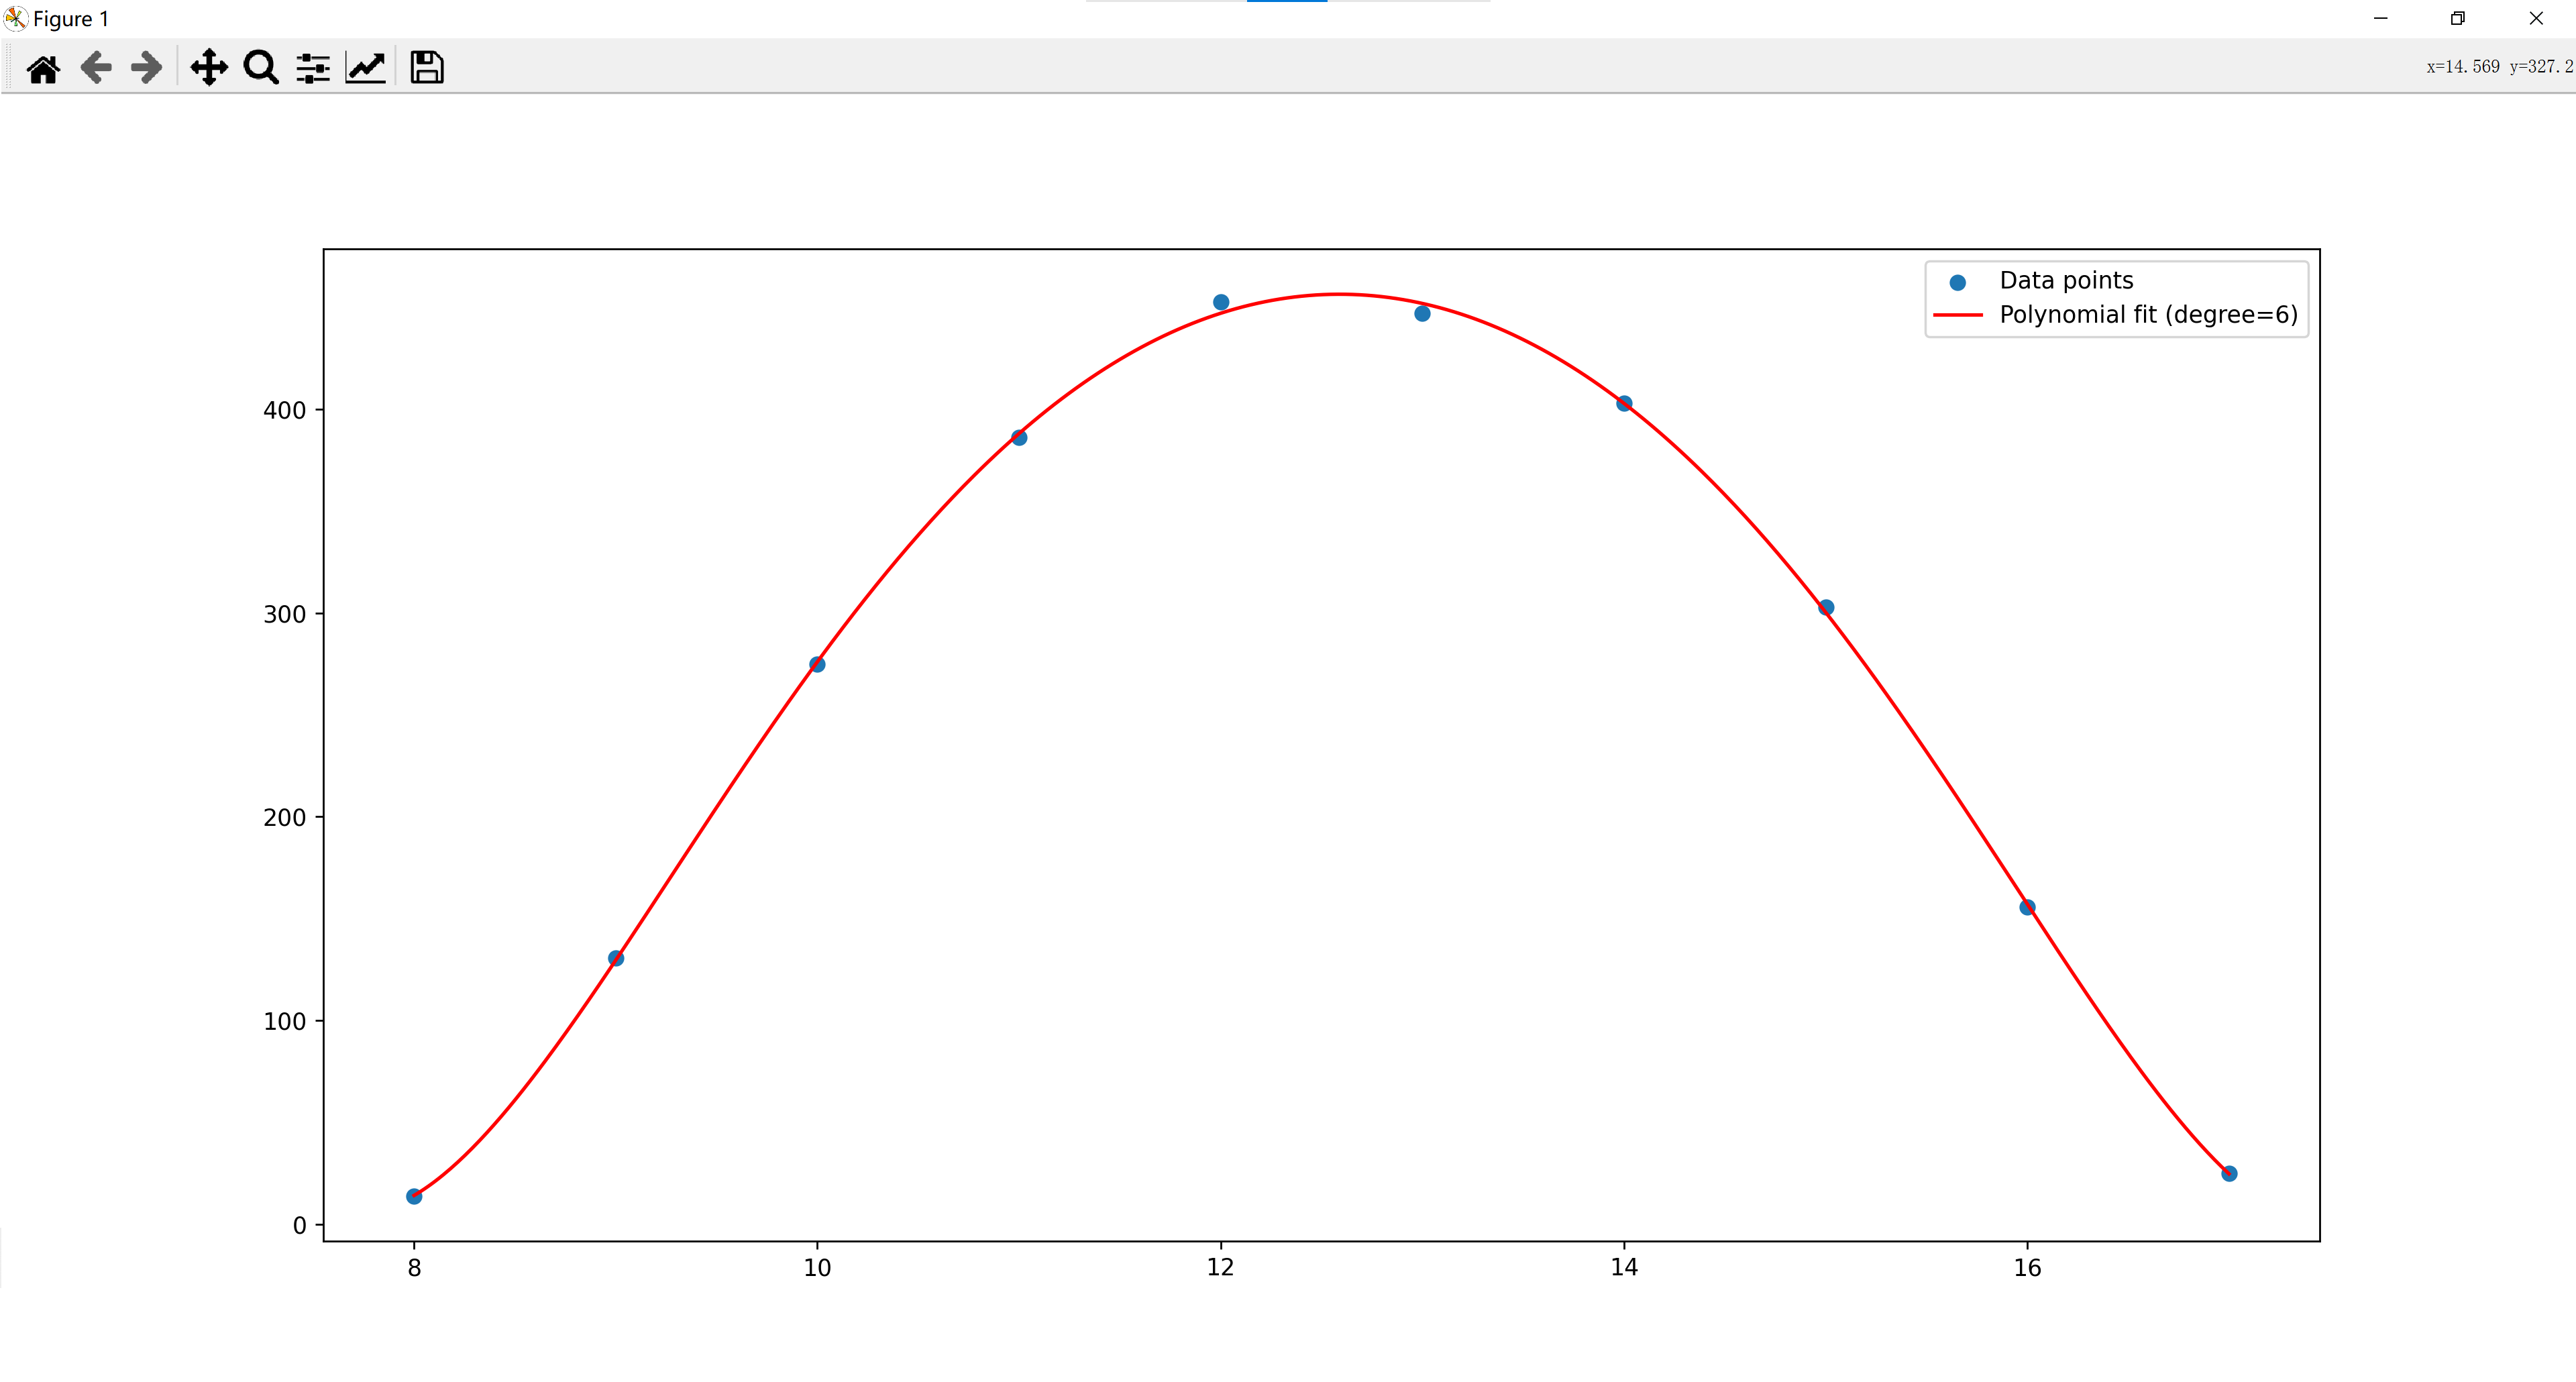
\includegraphics[width=0.8\textwidth]{"F:/Git/2012_B/papers/paper picture/good.png"} % 图片文件名及宽度调整
        \caption{这是一个图片示例} % 图片标题
        \label{fig:example} % 图片标签
    \end{figure}
    发现图线基本经过每一个离散点,证明拟合结果优良。
	\subsubsection{计算辐射量}
	利用积分,得出更加准确的辐射量。

    \subsubsection{最优太阳能电池板排布问题}
获得全年太阳能光伏发电总量尽可能大的前提是墙面获得最高的空间利用率。为此我们设计了一套算法。

\begin{itemize}
    \item $n_i$ 表示第 $i$ 种电池板的数量。
    \item $A_i$ 表示第 $i$ 种电池板的面积。
\end{itemize}

目标函数可以表示为:
\[
\max \left( \sum_{i} A_i \cdot n_i \right)
\]


1.使用嵌套循环在墙面区域内按一定间隔(电池板的长度和宽度)进行检查,尝试铺设电池板。

2.对每个可能的位置,检查电池板是否与排除区域重叠。

3.如果电池板位置有效(不重叠排除区域和其他已铺设电池板),则将其添加到布局中。
    \begin{figure}[H] % [H] 表示强制当前位置插入图片
        \centering % 使图片居中
        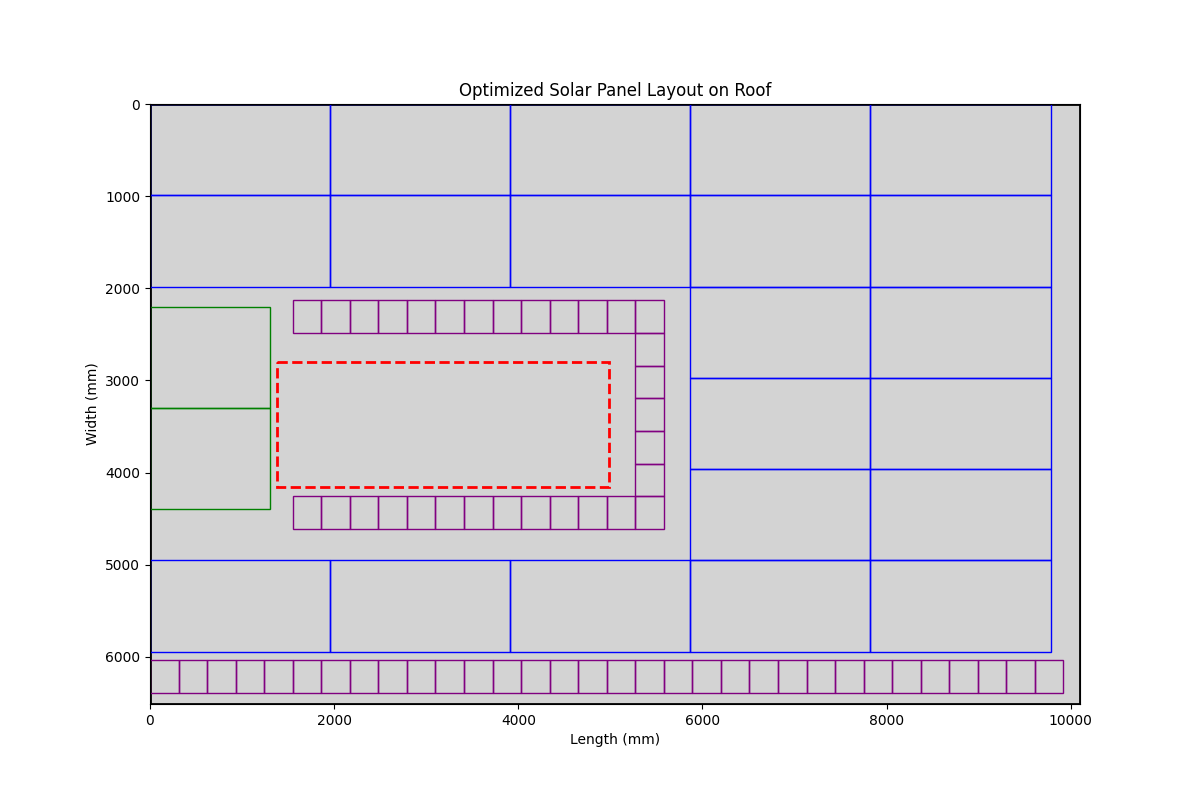
\includegraphics[width=0.8\textwidth]{"F:/Git/2012_B/papers/paper picture/south_top_B2_21_C1_2_C6_63.png"} % 图片文件名及宽度调整
        \caption{这是一个图片示例} % 图片标题
        \label{fig:example} % 图片标签
    \end{figure}

    \begin{figure}[H] % [H] 表示强制当前位置插入图片
        \centering % 使图片居中
        \includegraphics[width=0.5\textwidth]{example-image-a} % 图片文件名及宽度调整
        \caption{这是一个图片示例} % 图片标题
        \label{fig:example} % 图片标签
    \end{figure}


    
    \subsubsection{结果的检验}
    \subsubsection{问题的结论}
    \subsection{问题二模型的建立与求解}
    
    \subsubsection{某某模型的建立与求解}

    \subsubsection{结果的检验}
    \subsubsection{问题的结论}
    \subsection{问题三模型的建立与求解}
    \subsubsection{模型的建立}
    \subsubsection{模型的求解}
    \subsubsection{结果的检验}
    \subsubsection{问题的结论}
    \section{模型评价与改进}
    \subsection{模型优点}
    \begin{enumerate}[(1)]
        \item 针对第一问中,将原有的离散数据转为连续数据,在计算太阳光辐射时可以更加精确。
        \item 采用算法
    \end{enumerate}
    \subsection{模型缺点}
    \begin{enumerate}[(1)]
        \item 问题一中
        \item 结果
    \end{enumerate}

    \begin{thebibliography}{9} % 参考文献
		\bibitem{bib:8}何晓群.多元统计分析.北京:中国人民大学出版社,2012.
		\bibitem{bib:9}徐维超. 相关系数研究综述[J]. 广东工业大学学报,2012,29(3):12-17.
    \end{thebibliography}
    
    \newpage
    \section{附录}
    %插入代码内容
    \begin{lstlisting}
    \end{lstlisting}
\end{document}       